%% LyX 2.2.1 created this file.  For more info, see http://www.lyx.org/.
%% Do not edit unless you really know what you are doing.
\documentclass[spanish,english]{article}
\usepackage{lmodern}
\usepackage[T1]{fontenc}
\usepackage[latin9]{inputenc}
\setlength{\parskip}{\smallskipamount}
\setlength{\parindent}{0pt}
\usepackage{graphicx}
\usepackage{setspace}
\onehalfspacing

\makeatletter

%%%%%%%%%%%%%%%%%%%%%%%%%%%%%% LyX specific LaTeX commands.
%% Because html converters don't know tabularnewline
\providecommand{\tabularnewline}{\\}

\makeatother

\usepackage{babel}
\addto\shorthandsspanish{\spanishdeactivate{~<>}}

\usepackage{listings}
\addto\captionsenglish{\renewcommand{\lstlistingname}{Listing}}
\addto\captionsspanish{\renewcommand{\lstlistingname}{Listado de c�digo}}
\renewcommand{\lstlistingname}{Listing}

\begin{document}
\selectlanguage{spanish}%
\begin{center}
{\Large{}Costa Rica Institute of Technology}
\par\end{center}{\Large \par}

\medskip{}
\medskip{}

\begin{center}
{\Large{}Computer Engineering Academic Area}
\par\end{center}{\Large \par}

\medskip{}
\medskip{}

\begin{center}
{\Large{}Licentiate Degree Program in Computer Engineering}\medskip{}
\medskip{}
\par\end{center}

\begin{center}
\medskip{}
{\Large{}Course: CE-4303 \textendash{} Operating Systems Principles}\medskip{}
\par\end{center}

\begin{center}
\includegraphics{../../../../../Proyecto2/Documentacion/Documentation/images/logo_tec}
\par\end{center}

\begin{center}
\medskip{}
{\Large{}Project \#3: Robotic Finger}\medskip{}
\par\end{center}

\begin{center}
\medskip{}
 {\Large{}Made by:}\medskip{}
\par\end{center}

\begin{center}
\medskip{}
{\Large{}Daniel Gerardo Canessa Valverde, 201137483}
\par\end{center}{\Large \par}

\begin{center}
{\Large{}Felipe Alberto Mej�as Lor�a, 201231682}
\par\end{center}{\Large \par}

\begin{center}
{\Large{}Edward Uma�a Williams, 201128403}
\par\end{center}{\Large \par}

\begin{center}
\medskip{}
\par\end{center}

\begin{center}
\medskip{}
 {\Large{}Professor:}\medskip{}
\par\end{center}

\begin{center}
{\Large{}Jennifer Vargas Gonzalez.}\medskip{}
\par\end{center}

\begin{center}
\medskip{}
\medskip{}
 {\Large{}Date: November 15th, 2016}
\par\end{center}{\Large \par}

\pagebreak{}

\selectlanguage{english}%
\textbf{\Large{}Introduction }{\Large \par}

\textbf{\large{}Device drivers}{\large \par}

For the development of this project is important define some concepts,
these concepts are going to be used along of this document. Some of
the concepts are below:
\begin{itemize}
\item Process management: The kernel is in charge of creating and destroying
processes and handling their connection to the outside world. {[}1{]}
\item Memory management: The computer\textquoteright s memory is a major
resource, and the policy used to deal with it is a critical one for
system performance.{[}1{]}
\item Filesystems: Unix is heavily based on the filesystem concept; almost
everything in Unix can be treated as a file. {[}1{]}
\item Device control: Almost every system operation eventually maps to a
physical device. With the exception of the processor, memory, and
a very few other entities, any and all device control operations are
performed by code that is specific to the device being addressed.
That code is called a device driver. {[}1{]}
\item Networking: Networking must be managed by the operating system, because
most network operations are not specific to a process: incoming packets
are asynchronous events. {[}1{]}
\item Loadable modules: One of the good features of Linux is the ability
to extend at runtime the set of fea- tures offered by the kernel.
This means that you can add functionality to the kernel while the
system is up and running. Each piece of code that can be added to
the kernel at runtime is called a module. The Linux kernel offers
support for quite a few different types of modules, including, but
not limited to, device drivers. Each module is made up of object code
that can be dynamically linked to the run- ning kernel by the insmod
program and can be unlinked by the rmmod program. {[}1{]}
\end{itemize}
The Linux way of looking at devices distinguishes between three fundamental
device types. Each module usually implements one of these types, and
thus is classifiable as a char module, a block module, or a network
module. The three classes of modules are:
\begin{itemize}
\item Character devices: A character device is one that can be accessed
as a stream of bytes; a char driver is in charge of implementing this
behavior. Such a driver usu- ally implements at least the open, close,
read, and write system calls. The text console (/dev/console) and
the serial ports are examples of char devices, as they are well represented
by the stream abstraction. {[}1{]}
\item Block devices: Like char devices, block devices are accessed by filesystem
nodes in the /dev directory. A block device is a device that can host
a filesystem. In most Unix systems, a block device can only handle
I/O operations that transfer one or more whole blocks, which are usually
512 bytes in length. {[}1{]}
\item Network interfaces: Usually, an interface is a hardware device, but
it might also be a pure software device, like the loopback interface.
A network interface is in charge of sending and receiving data packets,
driven by the network subsystem of the kernel, without knowing how
individual transactions map to the actual packets being transmitted.{[}1{]}
\end{itemize}
Every USB device is driven by a USB module that works with the USB
subsystem, but the device itself shows up in the system as a char
device, a block device, or a network device. The Linux kernel supports
two main types of USB drivers: drivers on a host system and drivers
on a device. The USB drivers for a host system control the USB devices
that are plugged into it, from the host\textquoteright s point of
view. The USB drivers in a device, control how that single device
looks to the host computer as a USB device. The approach to writing
a USB device driver consist that the driver registers its driver object
with the USB subsystem and later uses vendor and device identifiers
to tell if its hardware has been installed. USB devices consist of
configurations, interfaces, and endpoints:
\begin{itemize}
\item Endpoints: The most basic form of USB communication is through something
called an endpoint. A USB endpoint can carry data in only one direction,
either from the host computer to the device or from the device to
the host computer.{[}1{]}
\item Interfaces: USB endpoints are bundled up into interfaces. USB interfaces
handle only one type of a USB logical connection, such as a mouse,
a keyboard, or a audio stream.{[}1{]}
\item Configurations: USB interfaces are themselves bundled up into configurations.
A USB device can have multiple configurations and might switch between
them in order to change the state of the device. {[}1{]}
\item USB Urbs: The USB code in the Linux kernel communicates with all USB
devices using something called a urb. This request block is described
with the struct urb structure and can be found in the include/linux/usb.h
file. A urb is used to send or receive data to or from a specific
USB endpoint on a specific USB device in an asynchronous manner. {[}1{]}
\end{itemize}
\textbf{\large{}Project specification}{\large \par}

The first part of the project is to create a robotic finger, using
any desired embedded device. Its a decision of the programmers to
choose the physical interface to interact with the computer, it can
be any of the following: USB, Parallel port, or communications port
(COM). This robotic finger will be used to automate physical tests
over a smart phone or tablet. It will be interacting with the screen
of the corresponding smart phone or tablet emulating a human finger.
The following kind of instructions are going to be available:
\begin{itemize}
\item Touch: on this kind of instruction the robotic finger will approach
the screen, touch the screen and then will reverse to its initial
position.
\item Push: on this kind of instruction, the robotic finger is going to
approach the screen and is going to touch it during a specified amount
of time, then it will reverse to its initial position.
\item Drag: on this kind of instruction, the robotic finger is going to
1) approach the screen, 2) is going to touch the screen and 3) move
the finger in any of the X and Y axes while the finger it's still
pushing the screen. Once done, 4) it will reverse the finger to its
original position.
\end{itemize}
The second part of the project consists in develop a device driver
in C programming language that will be working on any Linux Operating
System. This device driver will take care of providing to the upper
layers several primitives that will allow the interaction with the
physical device. 

The third part of the project consists in create a library in any
desired language. This library will allow the implementation of the
functions provided by the device driver, this means this library will
be the one interacting directly with the device driver specified in
the above point. It will be required to describe a common language
that will let us describe any of the instructions specified in section
A . This language will have to manage the following concepts:
\begin{itemize}
\item Instruction type (touch, push, drag).
\item X,Y initial position.
\item X,Y final position.
\end{itemize}
The fourth part of the project consists in develop a program that
will implement the small language just described and will make possible
the configuration/setup of the robotic finger.

The fifth part of the project consists in develop a physical test
program to test the robotic finger functionality. It will consists
of a numerical keyboard (similar to the one used by the BNCR in its
Internet banking). The software is going to generate a random PIN
of 6 digits and the robotic finger should type this PIN in order to
pass the physical test. The program is going to have several screen
resolutions:
\begin{itemize}
\item 1x1: This is the minimal screen resolution. It will divide the screen
in 1cmx1cm matrices. 
\item 2x2: It will divide the screen in 2cmx2cm matrices.
\item 4x4: It will divide the screen in 4cmx4cm matrices.
\end{itemize}
\selectlanguage{spanish}%
\pagebreak{}

\selectlanguage{english}%
\textbf{\Large{}Development environment}{\Large \par}
\begin{itemize}
\item The program was developed using Ubuntu 15.04. 
\item Sublime 3, this is a very popular code editor, besides give some tools
that makes the development of the code easier than other idles. 
\item GCC was used to compile the programs using the 6.1 version. 
\item Arduino Idle 1.6.7.
\item App Inventor 2.
\end{itemize}
\selectlanguage{spanish}%
\pagebreak{}

\selectlanguage{english}%
\textbf{\Large{}Continuous learning attribute analysis}{\Large \par}

We divided the project on 3 parts:
\begin{itemize}
\item Software: The software that handles the communication with the device,
is divided in three main blocks. The interpreter, the device library
and finally the device driver. All together allow a communication
with the hardware. First the interpreter, this block is in charge
of interpreting the instructions written on the config file, this
means that after reading the file , we should know the board size
and the differents moves to create complete the pin on the phone.
The interpreter use the device library which is the other big block,
this one have the methods that process the board information and the
diferentes moves that it can make, like drag , push or touch, those
both methods will send the information to the arduino using the last
block, the arduino driver. The arduino driver make the communication
with the physical device possible. This block read and write in the
device allowing the information of the board to be received by the
hardware. .
\item Hardware: To design the finger robot we use an ATMEGA 328 microcontroller,
because it give us the necessary ports for the servo motors, allowing
us to control the servos. To design the finger movement we base our
design to work like a CNC or a plotter. The servo motor are attached
to some roles which generates the movement. For the X and Y axes move,
the servo move a base in the corresponding direction. So this means
that the x servo moves his base and the Y axe base and the Y servo
moves only in his direction. For the Z axe, we attached a servo as
the X and Y cases, but in this case is placed vertically. So this
means that the phone is moving with the base in the X and Y direction
and the finger in the Z direction.
\item Physical test software: we decide to make an Android application using
the App Inventor tool, because the functionality of the application
is easy and because App Inventor give us all the necessary widgets
we need to develop the application. We decided to use Android because
all of us have Android smartphones, so we can make the tests with
our phones.
\end{itemize}
\selectlanguage{spanish}%
\pagebreak{}

\selectlanguage{english}%
\textbf{\Large{}Program design}{\Large \par}

\textbf{\large{}USB driver code}{\large \par}

The development team have tried to use the best programming practices,
in this way the code reutilization was fundamental in this project
building. The project contains the following common files: USBDriver.c,
ArduinoDriverLibrary.h. The description of this files is as follows:
\begin{itemize}
\item USBDriver.c: this file contains all the structures, interfaces and
functions of the USB driver. 
\item ArduinoDriverLibrary.h: this file contains all the functions that
interacts with the USB driver functions. 
\end{itemize}
USBDriver.c have the following methods:
\begin{itemize}
\item static int usb\_open(struct inode {*}inode, struct file {*}file):
This method is going to open the file corresponding with the Arduino.
\item static void usb\_delete(struct kref {*}kref): This method is going
to create the structure that contains all of the data need it on one
side of the bride.
\item static ssize\_t usb\_read(struct file {*}file, char \_\_user {*}buffer,
size\_t count, loff\_t {*}ppos): This function is use to read information
send by the device.
\item static void usb\_write\_bulk\_callback(struct urb {*}urb): After the
urb is successfully transmitted to the USB device, this function is
called by the USB core.
\item static ssize\_t usb\_write(struct file {*}file, const char \_\_user
{*}user\_buffer, size\_t count, loff\_t {*}ppos): This function is
in charged of write data to the device.
\item static int usb\_probe(struct usb\_interface {*}interface, const struct
usb\_device\_id {*}id): The probe function is called when a device
is installed that the USB core thinks this driver should handle; the
probe function should perform checks on the information passed to
it about the device and decide whether the driver is really appropriate
for that device.
\item static void usb\_disconnect(struct usb\_interface {*}interface): The
disconnect function is called when the driver should no longer control
the device for some reason and can do clean-up.
\item static int \_\_init usb\_init(void): This functions is in charged
of register the USB driver.
\item static void \_\_exit usb\_exit(void): This function is in charged
of unregister the USB driver.
\end{itemize}
ArduinoDriverLibrary.h have the following methods:
\begin{itemize}
\item int send\_message\_to\_arduino (char stringToSend{[}256{]}): This
function is going to send a message to the arduino file.
\item char{*} read\_message\_send\_from\_arduino(): This function is going
to read a message send from the arduino.
\end{itemize}
\textbf{\Large{}Android application}{\Large \par}

For the physical test program, we develop an Android app with the
following functions:
\begin{itemize}
\item checkPin: this method is in charge of check if the pin introduced
by the robotic finger is correct.
\item concatenatePin: this method is in charge of update the pin introduced
by the robotic finger.
\end{itemize}
\textbf{\Large{}Interpreter}{\Large \par}

The interpreter was developed in C programing languaje. The interpreter
reads an file called config.txt, this file is the input of the interpreter,
in this file there are some instructions compatible con the interpreter,
the interpreter reads the instructions, for each instruction it detects
what kind is this and descompose it, finally the interpreter generates
his output, that is call the appropiate method of the device library,
that is going to handle the descompose instruction.

There are two types of instruction, the board instruction and the
move instruction.
\begin{itemize}
\item Board instruction: this type of instruction indicates the size of
the board.
\item Move instruction: this type of instruction indicates the kind of movement
(push, drag, touch), the current position of the robotic finger and
the final position of the robotic finger (target position).
\end{itemize}
The interpreter is composed by 4 methods, these methods are described
below:
\begin{itemize}
\item findSubstr: this method receibe a char array and a pattern, it return
the position where the pattern is find in the array.
\item str\_split: this method receibe a char array, split the array in chars
and return a list of arrays.
\item processMove: this method gets the information of the movement and
call the device library.
\item processBoard: this method gets the information of the board and call
the device library.
\end{itemize}
\textbf{\Large{}Device Library}{\Large \par}

The device library was developed in C programing language. The device
library has an input from the interpreter and comunicates with the
device driver like an output. The device library is composed by 2
methods, these methods are described below:
\begin{itemize}
\item processMoveDevice: this method call the device driver, it sends nextMove:
1 if the move is touch, 2 if the move is push, 3 if the move is drag,
posFin and posIni a number in the range 0-9.
\item processBoardDevice: this method call the device driver, it sends size
board: 1 if the board is 1x1, 2 if the board is 2x2, 3 if the board
is 4x4. 
\end{itemize}
\textbf{\Large{}Language}{\Large \par}

The language designed to control the interpreter have the syntax ``type\_instruction
-parameters'', the specification is as follows:

Setting the board:
\begin{itemize}
\item board -b sizeBoard, where size board can be 1x1, 2x2 or 3x3
\end{itemize}
Doing a movement:
\begin{itemize}
\item move -t typeofmovement -i initialPosition -f finalPosition, where
typeofmovement can be touch, drag or push, initialPosition can be
an integer in the range of 0-9, finalPosition can be an integer in
the range of 0-9.
\end{itemize}
\textbf{\Large{}Arduino code}{\Large \par}

For the arduino code, we have this two methods that get how much they
have to move using the formula |posIni - posFin|{*}separation, so
with this formula the servo will know how much to move.

\begin{lstlisting}
void moveX(int posIni, int posFin, int separation)
void moveY(int posIni, int posFin, int separation).
\end{lstlisting}

The arduino use this method to create the Z movement, the dir parameter
means if is going up or down.

\begin{lstlisting}
void moveZ(int dir).
\end{lstlisting}

The arduino use the cast method to simplify the matrix, so it map
the position and return a generic position.

\begin{lstlisting}
int castNumberY(int number) 
int castNumberX(int number)
\end{lstlisting}

The arduino reads the information coming for the device library.

\begin{lstlisting}
void serialEvent()
\end{lstlisting}

\textbf{\large{}\pagebreak{}UML Diagram} 

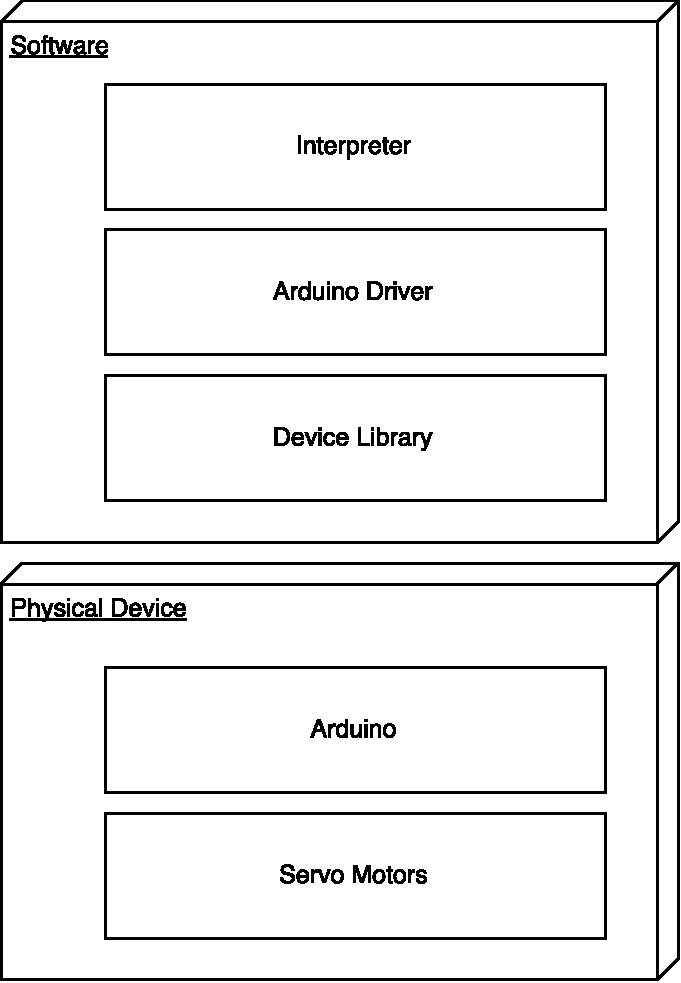
\includegraphics[scale=0.5]{images/operativos}

Figure 1. UML Diagram 

\textbf{\large{}\newpage{}Diagrams of the physical simulation}

To design the finger robot we use an ATMEGA 328 microcontroller, because
it give us the necessary ports for the servo motors, allowing us to
control the servos. To design the finger movement we base our design
to work like a CNC or a plotter. The servo motor are attached to some
roles which generates the movement. 

For the X and Y axes move, the servo move a base in the corresponding
direction. So this means that the x servo moves his base and the Y
axe base and the Y servo moves only in his direction. For the Z axe,
we attached a servo as the X and Y cases, but in this case is placed
vertically. So this means that the phone is moving with the base in
the X and Y direction and the finger in the Z direction.

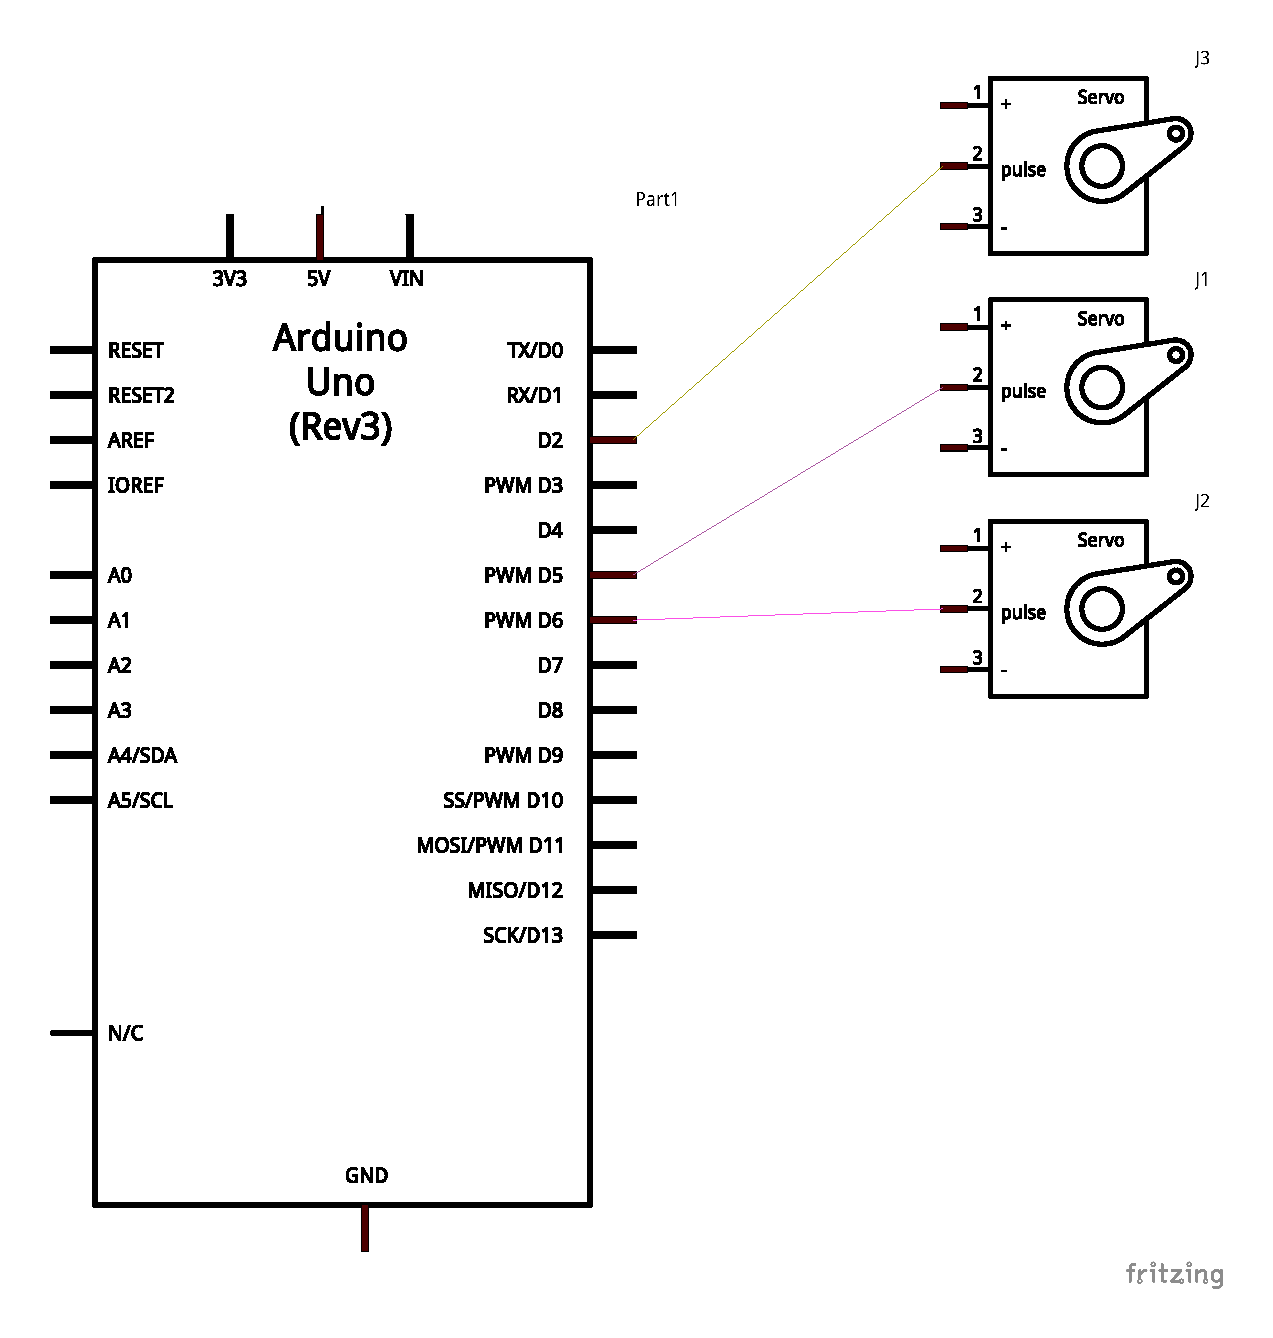
\includegraphics[scale=0.5]{images/operativos_schem}

Figure 2. Schematic Diagram of the physical simulation

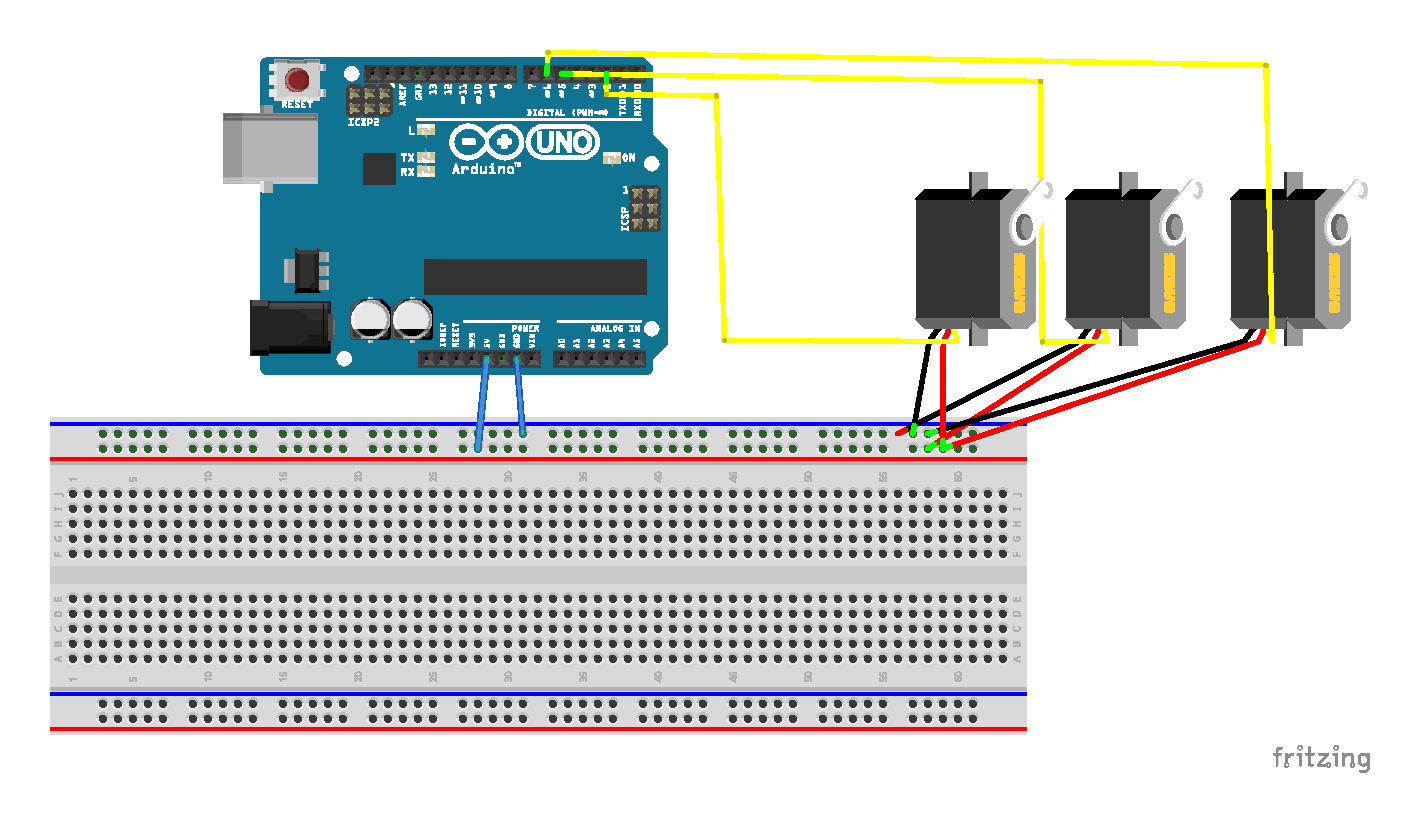
\includegraphics[scale=0.5]{images/operativos_bb}

Figure 3. Arduino diagram of the physical simulation

\selectlanguage{spanish}%
\pagebreak{}

\selectlanguage{english}%
\textbf{\Large{}Instructions of how to use the program}{\Large \par}
\begin{enumerate}
\item Compile the project using the command make. In the root folder. This
will create an executable called Interpreter.
\item Run the script that configure the driver, place in the root folder
and write in terminal \$sh mountDriver.sh
\item To run the project use the follow line on the terminal. \$./Interpreter
configFile, where configFile, represents the file that have all the
instructions to execute.
\end{enumerate}

\selectlanguage{spanish}%
\pagebreak{}

\selectlanguage{english}%
\textbf{\Large{}Student activity log}{\Large \par}

Daniels Activity Log

\begin{tabular}{|c|c|c|}
\hline 
Date & Hours & Activity\tabularnewline
\hline 
\hline 
5/11/2016 & 7 & Interpreter Development\tabularnewline
\hline 
6/11/2016 & 8 & Interpreter Development\tabularnewline
\hline 
9/11/2016 & 4 & Device Library Deveploment\tabularnewline
\hline 
10/11/2016 & 4 & Device Library Deveploment\tabularnewline
\hline 
11/11/2016 & 8 & Arduino Software\tabularnewline
\hline 
12/11/2016 & 5 & Arduino Software\tabularnewline
\hline 
14/11/2016 & 8 & Calibration\tabularnewline
\hline 
15/11/2016 & 6 & Documentation\tabularnewline
\hline 
Total & 50h & \tabularnewline
\hline 
\end{tabular}

Edwards Activity Log

\begin{tabular}{|c|c|c|}
\hline 
Date & Hours & Activity\tabularnewline
\hline 
\hline 
6/11/2016 & 6 & Finger Physical Device Investigation\tabularnewline
\hline 
9/11/2016 & 8 & Finger Physical Investigation and buying materials\tabularnewline
\hline 
10/11/2016 & 6 & Using servo motors to move rols\tabularnewline
\hline 
11/11/2016 & 15 & Creating the CNC model\tabularnewline
\hline 
12/11/2016 & 8 & Using the Machine with the drivers\tabularnewline
\hline 
14/11/2016 & 6 & Making the Z movement\tabularnewline
\hline 
Total & 49h & \tabularnewline
\hline 
\end{tabular}

Felipes Activity Log

\begin{tabular}{|c|c|c|}
\hline 
Date & Hours & Activity\tabularnewline
\hline 
\hline 
05/11/2016 & 11 & Driver Investigation\tabularnewline
\hline 
06/11/2016 & 11 & Driver Investigation and Implementation\tabularnewline
\hline 
09/11/2016 & 3 & Robotic Finger Design\tabularnewline
\hline 
11/11/2016 & 6 & USB Driver and Arduino communication\tabularnewline
\hline 
12/11/2016 & 6 & Robotic Finger communication and application design\tabularnewline
\hline 
14/11/2016 & 5 & Physical test software and Robotic Finger test\tabularnewline
\hline 
15/11/2016 & 6 & Documentation and testing\tabularnewline
\hline 
Total & 48h & \tabularnewline
\hline 
\end{tabular}

\selectlanguage{spanish}%
\pagebreak{}

\selectlanguage{english}%
\textbf{\Large{}Project final status}{\Large \par}

The project is completed satisfactorily, the only issue is the board
of 4x4 have a size that exceed the phone screen size, for this reazon
we can't show the correct funtionability, but all the software and
hardware support this board.

\textbf{\Large{}Conclusions }{\Large \par}
\begin{itemize}
\item All the USB drivers needs a \textquotedblleft char\textquotedblright{}
or \textquotedblleft block\textquotedblright{} interface to communicate
with the program in the user space.
\item The endpoints of a device determinate if the USB is an output or input,
and you cand send bulk or interrupt information to them.
\item Using a library abstract the programs how the hardware works and improve
the efficiency of using that hardware.
\end{itemize}
\textbf{\Large{}Recommendations}{\Large \par}
\begin{itemize}
\item The generic CNC design allows an excellent 3 dimensional movement. 
\item To avoid the friction created by the wood and steel pieces is recommended
to increase the roles in the axes, taking in mind that this will increase
the project price.
\item It's important to unmount the driver of the device, before mount your
driver for that same device.
\item Create a script that unmount and mount the drivers , this will make
it easier to use.
\end{itemize}
\selectlanguage{spanish}%
\pagebreak{}

\selectlanguage{english}%
\textbf{\Large{}References}{\Large \par}

{[}1{]} A. Rubini and J. Corbet, Linux device drivers, 1st ed. Sebastopol:
O'Reilly \& Associates, 2001.
\end{document}
